\documentclass[tikz]{standalone}
\usepackage{pgfplots}
\usepackage{mathpazo}
\usepgfplotslibrary{polar}
\usepgflibrary{shapes.geometric}
\usetikzlibrary{calc}
\usetikzlibrary{datavisualization}
\usetikzlibrary{datavisualization.formats.functions}
\pgfplotsset{compat=1.12} 
\pgfplotsset{my style/.append style={axis x line=middle, axis y line=middle, xlabel={$x$},ylabel={$y$},smooth}}
\begin{document}
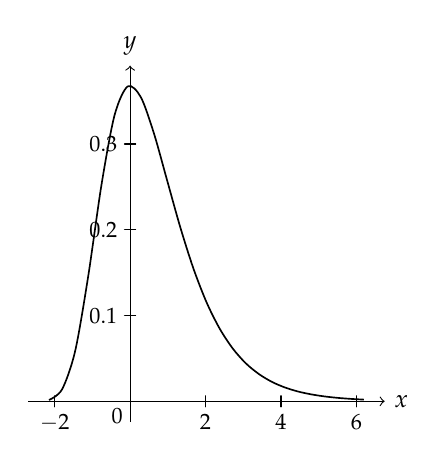
\begin{tikzpicture}[scale=1]
\datavisualization [school book axes, visualize as smooth line/.list={normal},all axes = {length=4cm,ticks = some},x axis ={label=$x$},y axis ={label=$y$}]
%,normal={pin in data={text=$y{=}e^{-x}e^{-e^{-x}}$,when=x is 0.5}}]
data [format=function] {
var x : interval [-2.15:6.2];
func y = exp(-\value x)*exp(-exp(-\value x));
};
\end{tikzpicture}
\end{document}